\documentclass{article}


\usepackage{arxiv}

\usepackage[utf8]{inputenc} % allow utf-8 input
\usepackage[T1]{fontenc}    % use 8-bit T1 fonts
\usepackage{hyperref}       % hyperlinks
\usepackage{url}            % simple URL typesetting
\usepackage{booktabs}       % professional-quality tables
\usepackage{amsfonts}       % blackboard math symbols
\usepackage{nicefrac}       % compact symbols for 1/2, etc.
\usepackage{microtype}      % microtypography
\usepackage{mathtools} 

\usepackage{graphicx}
\graphicspath{ {./images/} }

\title{DroneNet: using drone swarms for autonomous search and rescue}


\author{
  Jacky Zhao
  St. George's School\\
  Vancouver, CA\\
  \texttt{j.zhao2k19@gmail.com} \\
}

\begin{document}
\maketitle

\begin{abstract}
\texttt{
Current search and rescue methods are very reliant on global communication methods like GPS or a central control unit. This limits the range and efficiency of search and rescue operations. A decentralized drone swarm would alleviate these problems by having a theoretically infinite range given number of drones. So far, I have designed and assembled the first drone using 3D printed components and ordered parts, built the recognition network by retraining a YOLOv3 model on the COCO and KITTI datasets. The next component would be to implement the decentralized autopilot using a Deep Q-learning Agent or another reinforcement learning algorithm to output velocity deltas. 
} \\
\end{abstract}


\section{Introduction}
Search and rescue (SAR) operations are some of the most important in the world, saving thousands of lives each year. However, SAR operations are severely hampered by the 'searching' aspect of SAR. THis is due to several factors, namely 1. speed of the operation, and 2. accuracy of detection. Firstly, many, if not most, SAR operations are conducted on foot or via helicopter. However, while on-foot operations are more accurate, they lack the speed to be very effective. Helicopter operations, on the other hand, are fast but are often prone to low accuracy. There have been many efforts to address this lack of a better solution, including proposals to use OpenCV and neural networks in drones for improved performance in the human-identification process. However, this improvement is still marginal as only one drone is being used at a time. Institutions such as MIT have proposed solutions which involve controlling a drone swarm for increased efficiency. Interestingly, there has been no published attempt at completing a project which involves creating both the human-detection and drone swarm management algorithms.

\section{Proposal}
\label{sec:headings}
I propose a novel end-to-end algorithm for controlling drone swarms for autonomous search and rescue. This algorithms would be able to

\begin{enumerate}
  \item Efficiently navigate a 3D search space,
  \item Effectively communicate between an undetermined amount of drones and transfer data (location, images),
  \item Detect and identify humans
\end{enumerate}

As this task is extremely difficult, I plan to tackle this task in multiple stages. In the first stage, I plan to create a singular functioning drone which is able to navigate a 2D air space above a clear area, and efficiently find a human. 

\subsection{Hardware}
\subsubsection{Frame}
The physical frame of the drone is a modified build of the Firefly 1504 Drone. The mainframe is modified by first expanding the width to be able to fit the battery. Bumper\_v2\_f.stl and 2x side.stld is printed with 50\% infill. Lower\_plate\_V2.stl, Top\_plate\_front\_3mm.stl, and Top\_plate\_rear\_3mm.stl are printed with 25\% infill. Arms are 100mm segments of Carbon Fiber tube with a radius of 6mm. Holes and screws were drilled and assembled as according to the documentation of the Firefly.

\subsubsection{Cost and Equipment Breakdown}
The breakdown of the price and weight data for the construction of the first drone is listed below.
\begin{table}[h!]
\centering
\begin{tabular}{|l|l|l|l|}
\hline
Quantity & Item                                    & Total Weight (g) & Price    \\ \hline
1x       & 3D Printed Frame                        & 50.0g            & N/A      \\ \hline
1x       & 1300mAh 4S 45C LiPo Battery             & 165.0g           & \$19.10  \\ \hline
4x       & 20A 2-4S ESC                            & 28.0g            & \$50.68  \\ \hline
1x       & HobbyKing Lite Power Distribution Board & 19.3g            & \$4.13   \\ \hline
4x       & 100mm x 6mm Carbon Fiber Tubes          & 45.2g            & \$7.99   \\ \hline
1x       & PXFMini Power Module                    & 50.0g            & \$44.94  \\ \hline
1x       & PXFMini                                 & 15.0g            & \$103.36 \\ \hline
4x       & EMAX RS2205 Brushless Motor             & 120.0g           & \$39.96  \\ \hline
4x       & GEMFAN 5045 GRP 3-BLADE Propellers      & 21.2g            & \$8.76   \\ \hline
1x       & Pi Zero W                               & 9.0g             & \$5.00   \\ \hline
1x       & Pi Camera v1 5MP                        & 18.1g            & \$14.99  \\ \hline
N/A      & Misc. wires, bolts, and nuts            & 20.0g            & N/A      \\ \hline
Totals   & N/A                                     & 560.8g           & \$298.91 \\ \hline
\end{tabular}
\caption{Price and Weight Breakdown}
\end{table}

\subsubsection{Flight}
In calculating the thrust required, I consider that the drone will not be used for racing. As a result, a thrust to weight ratio of 4:1 works well. Using the weight of the drone calculated in 2.1.2, we get a thrust requirement of 2.43kg. Dividing this by the 4 motors, we require 560g of thrust per motor. I decided on using the GEMFAN 5045 propellers (5" diameter, 4.5" pitch). This allows the drone to achieve a thrust of roughly 560g per motor at only 13A draw or 52A total. 

\begin{table}[h!]
\centering
\begin{tabular}{|l|l|l|l|}
\hline
Current (A) & Thrust (g) & Efficiency (g/W) & Speed (RPM) \\ \hline
1           & 76         & 4.75             & 7220        \\ \hline
3           & 183        & 3.81             & 10790       \\ \hline
5           & 282        & 3.54             & 13030       \\ \hline
7           & 352        & 3.10             & 14720       \\ \hline
9           & 426        & 2.93             & 16180       \\ \hline
11          & 497        & 2.82             & 17150       \\ \hline
13          & 560        & 2.69             & 18460       \\ \hline
15          & 628        & 2.62             & 19270       \\ \hline
...         & ...        & ...              & ...         \\ \hline
27          & 997        & 2.28             & 23920       \\ \hline
30          & 1024       & 2.14             & 24560       \\ \hline
\end{tabular}
\caption{Thrust Table for RS2205-2300KV @ 16.8V with GF5045BN}
\end{table}

As such, I needed to choose a battery that would allow reasonable flight time given our 52A draw. We can use the Maximum Recommended Current Draw function which is as follows
\begin{equation}
I_{max} = Capacity_{Ah} \cdot C Rating
\end{equation}

For this project, a 1300mAh 4S 45C LiPo Battery was used. 

\[
I_{max} = 1.3Ah \cdot 4C = 58.5A
\]

This max current is greater than the maximum theoretical usage, thus, this battery is safe to use. Using this information, we can calculate the theoretical maximum flight time. To keep the drone in the air, we require approximately thrust equal to the weight of the drone (560g). This translates to roughly $140g$ of thrust per motor. I assume that the capacity is only 80\% effective, meaning $1.04Ah$ is available. We can then convert to minutes by multiplying by $h/60min$ and dividing by the current draw of $3A$. This attains a total flight time of 20.8 minutes.  

\subsubsection{Positioning}
A PXFMini is used as the data sensor hub and auto-pilot shield. This shield runs on top of the Raspberry Pi Zero W and allows the drone to be controlled using the APM flight stack. The PXFMini is able to get data such as height, global position, velocity, and acceleration. The APM outputs through the PWM Outputs on the back of the PXFMini.

\subsubsection{Communications}
Two main options are available for communication, WiFi and Radio. WiFi communication is achieved by connecting the Raspberry Pi Zero W to a local Wireless Access Point (WAP) hosted on my laptop. Two network interfaces are used. The Asus AC56R Wifi Adapter (rtl8812au driver) is used for WiFi Access while the Builtin Intel Wifi Adapter is used for creating wireless access point. The RPi attempts to start the ArduCopter APM at port 6000 with a UDP link. However, at this point in time, the APM Planner 2 program on my laptop refuses to connect to the port. For now, I will be resorting to traditional RC methods. Currently, I am using a RC controller with a PPMSUM-enabled receiver attached to the PXFMini. 

\subsection{Software}
\subsubsection{Detection Network}
The detection network is tasked with identifying and labelling humans within images taken by the Raspberry Pi Camera. The Tiny YOLOv1 Architecture was chosen for this task as it is has a very quick runtime ($\sim$30ms) on a 970M. Other options such as Full YOLOv1 and SqueezeNet were either too large or took too long to run a image. The architecture was implemented using Tensorflow v1.2.1 modified to run with a [448, 448, 3] dimensional input. Training was done on a combination of the KITTI and COCO datasets. Performance will be detailed at a later date.

\begin{figure}[h!]
  \caption{Tiny YOLOv1 Architecture}
  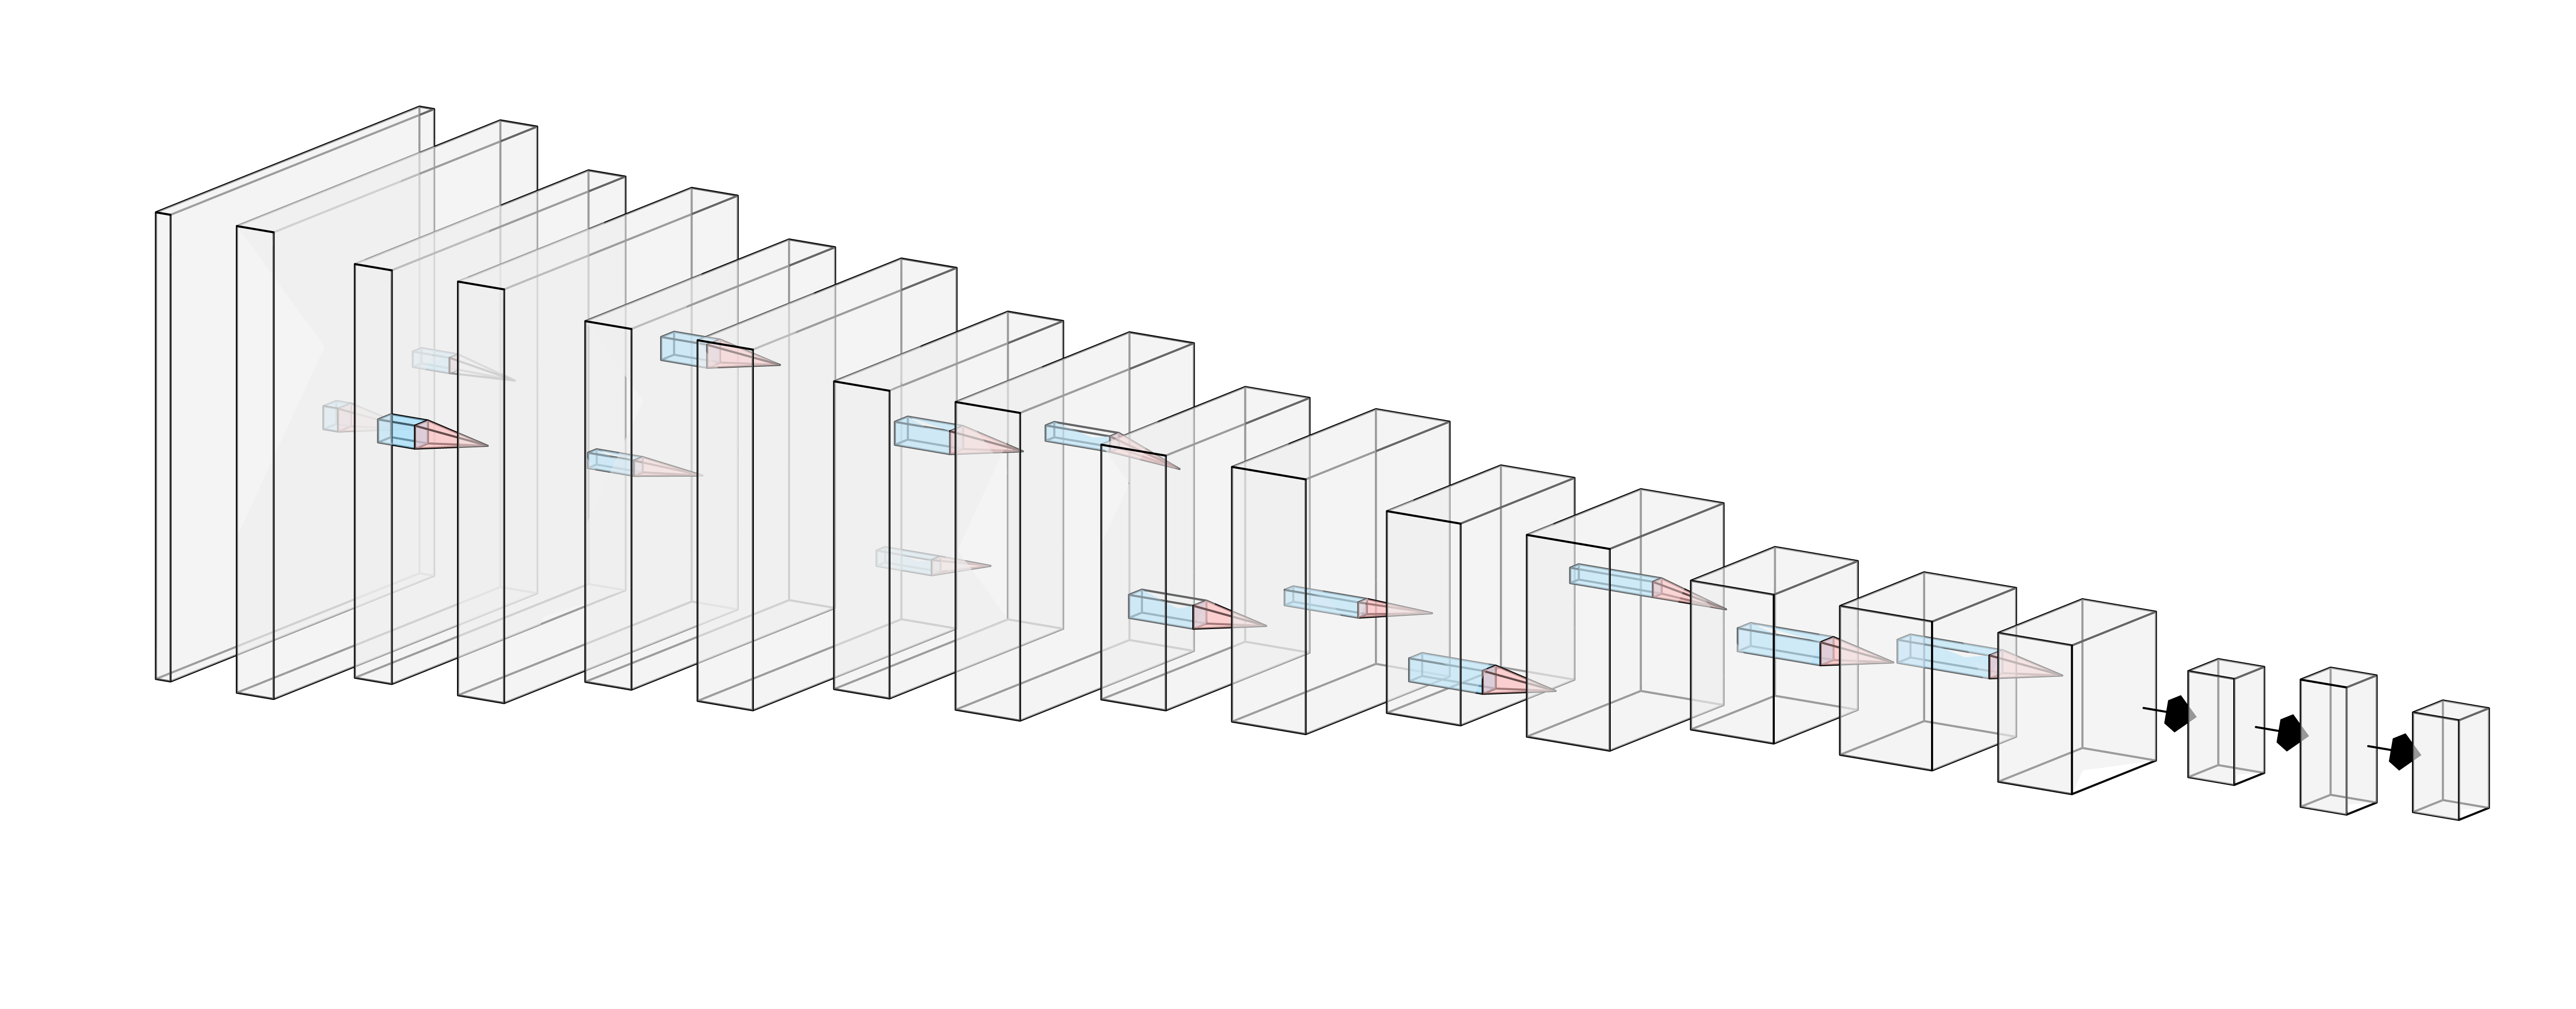
\includegraphics[width=\textwidth]{nn}
\end{figure}

The dimensions of each layer are determined by that of the layer before $N_n$, the kernel size $K$ and the stride length $S$.

\begin{equation}
N_n = \frac{N_{n-1} - K}{S} + 1
\end{equation}



\begin{table}[h!]
\centering
\begin{tabular}{|l|l|l|l|l|}
\hline
Layer    & Output Dimensions  & Filter Size & Stride     & Depth        \\ \hline
images   & {[}448, 448, 3{]}  & -           & -          & -            \\ \hline
conv1    & {[}448, 448, 16{]} & {[}3, 3{]}  & {[}1, 1{]} & 16           \\ \hline
maxpool1 & {[}224, 224, 16{]} & {[}2, 2{]}  & {[}2, 2{]} & -            \\ \hline
conv2    & {[}224, 224, 32{]} & {[}3, 3{]}  & {[}1, 1{]} & 32           \\ \hline
maxpool2 & {[}112, 112, 32{]} & {[}2, 2{]}  & {[}2, 2{]} & -            \\ \hline
conv3    & {[}112, 112, 64{]} & {[}3, 3{]}  & {[}1, 1{]} & 64           \\ \hline
maxpool3 & {[}56, 56, 64{]}   & {[}2, 2{]}  & {[}2, 2{]} & -            \\ \hline
conv4    & {[}56, 56, 128{]}  & {[}3, 3{]}  & {[}1, 1{]} & 128          \\ \hline
maxpool4 & {[}28, 28, 256{]}  & {[}2, 2{]}  & {[}2, 2{]} & -            \\ \hline
conv5    & {[}28, 28, 256{]}  & {[}3, 3{]}  & {[}1, 1{]} & 256          \\ \hline
maxpool5 & {[}14, 14, 256{]}  & {[}2, 2{]}  & {[}2, 2{]} & -            \\ \hline
conv6    & {[}14, 14, 512{]}  & {[}3, 3{]}  & {[}1, 1{]} & 512          \\ \hline
maxpool6 & {[}7, 7, 512{]}    & {[}2, 2{]}  & {[}2, 2{]} & -            \\ \hline
conv7    & {[}7, 7, 1024{]}   & {[}3, 3{]}  & {[}1, 1{]} & 1024         \\ \hline
conv8    & {[}7, 7, 256{]}    & {[}3, 3{]}  & {[}1, 1{]} & 256          \\ \hline
conv9    & {[}7, 7, 512{]}    & {[}3, 3{]}  & {[}1, 1{]} & 512          \\ \hline
fc1      & {[}1024{]}         & -           & -          & -1 (flatten) \\ \hline
fc2      & {[}4096{]}         & -           & -          & -            \\ \hline
fc3      & {[}675{]}          & -           & -          & -            \\ \hline
\end{tabular}
\caption{DetectionNet Architecture}
\end{table}

\begin{equation}
loss = \lambda_{obj}(loss_{dims} + loss_{objconf}  + loss_{prob}) + \lambda_{noobj}(loss_{noobjconf})
\end{equation} 

We define two constants that help to correct the unbalance between obj and no\_obj boxes, $\lambda_{obj}$ and $\lambda_{noobj}$. We set these to \textit{5.0} and \textit{0.5} respectively.

\begin{equation}
\phi_{i,j,h}^{obj} =
\begin{cases}
0 & \text{if object is in cell \textit{i,j} and bounding box \textit{h} is responsible} \\
1 & \text{otherwise}
\end{cases}
\end{equation}

\textit{sx, sy} are defined as number of horizontal grid cells and vertical grid cells, respectively classes is the list of total possible classes. \textit{B} is the number of bounding boxes per grid cell. $\delta$ is defined as a small constant to prevent extremely small numbers.

\begin{equation}
loss_{dims} = \sum\limits_{i=0}^{s_x}\sum\limits_{j=0}^{s_y}\sum\limits_{h=0}^{B}\phi_{i,j,h}^{obj}[(x_{i,j} - \hat{x}_{i,j})^2 + (y_{i,j} - \hat{y}_{i,j})^2 + (\sqrt{w_{i,j} + \delta} - \sqrt{\hat{w_{i,j}} + \delta})^2 + (\sqrt{h_{i,j} + \delta} - \sqrt{\hat{h_{i,j}} + \delta})^2]
\end{equation}

\begin{equation}
loss_{objconf} = \sum\limits_{i=0}^{s_x}\sum\limits_{j=0}^{s_y}\sum\limits_{h=0}^{B}\phi_{i,j,h}^{obj}(conf_{i,j} - \hat{conf}_{i,j})^2
\end{equation}

\begin{equation}
loss_{noobjconf} = \sum\limits_{i=0}^{s_x}\sum\limits_{j=0}^{s_y}\sum\limits_{h=0}^{B}\phi_{i,j,h}^{noobj}(conf_{i,j} - \hat{conf}_{i,j})^2
\end{equation}

\begin{equation}
loss_{prob} = \sum\limits_{i=0}^{s_x}\sum\limits_{j=0}^{s_y}\sum\limits_{c\in classes}^{}\phi_{i,j,h}^{noobj}(p(c)_{i,j} - \hat{p(c)}_{i,j})^2
\end{equation}




\subsubsection{Navigation Network}

\end{document}